\chapter{تست سامانه}

بعد از فصل پیاده‌سازی، این فصل به تست سامانه می‌پردازد. برای تست سامانه، موارد آزمون\LTRfootnote{\lr{Test case}} برای دو دسته نیازمندی‌های کارکردی و غیرکارکردی نوشته شده و هریک به صورت جداگانه بررسی می‌شود. در ادامه در بخش‌های تست نیازمندی‌های کارکردی و غیرکارکردی به موارد آزمون، برای هر نیازمندی به تفکیک پرداخته می‌شود.

\section{تست نیازمندی‌های کارکردی}

\subsection{تست کشف شبکه}
برای تست کشف شبکه با استفاده از ماشین‌های مجازی\LTRfootnote{\lr{Virtual Machine (VM)}} و سوئیچ‌های مجازی\LTRfootnote{\lr{Virtual Switch}}، شبکه‌ای طبق \cref{fig.51} طراحی شد. حال توسط ماشین مجازی که سامانه درحال اجرای آن است، کشف شبکه صورت می‌گیرد. نتیجه آن در \cref{fig.52} قابل مشاهده است.


\begin{figure}[!h]
    \centering\includegraphics[scale=.38]{./topo-test}
    \caption{تصویر توپولوژی شبکه‌ای جهت تست}\label{fig.51}
\end{figure}


\begin{figure}[!h]
    \centering\includegraphics[scale=.38]{./topo-test-result}
    \caption{تصویر توپولوژی بدست آمده از سامانه}\label{fig.52}
\end{figure}




\cleardoublepage

همانطور که مشاهده می‌شود، نتیجه بدست آمده با توپولوژی طراحی شده از قبل کاملا مطابقت می‌نماید.

\subsection{تست تنظیمات شبکه}

برای این بخش امکانی فراهم شده تا کاربر هنگام پایش اطلاعات شبکه، مواردی که در بخش تنظیمات ذخیره کرده است را مشاهده می‌کند (\cref{fig.18}).


\subsection{تست پردازش و ذخیره اطلاعات جمع‌آوری شده}

این تست از دو بخش تشکیل می‌شود:

\begin{itemize}
    \item نمایش نمودارهای پایش عملکرد عنصر تحت مدیریت
    \item نمایش اطلاعات قدیمی در صورت پایش قبلی
\end{itemize}

برای بخش اول \cref{fig.53} کفایت می‌کند، چون نمودارها به صورت بی‌درنگ درحال نمایش اطلاعات دریافتی هستند.


برای بخش دوم نیز دوباره بعد از بستن تب موردنظر دوباره اقدام به پایش کرده که نتیجه آن در \cref{fig.54} قابل مشاهده است. درواقع اطلاعات قدیمی از ردیس بازیابی شده و نمایش داده می‌شود.


\begin{figure}[!h]
    \centering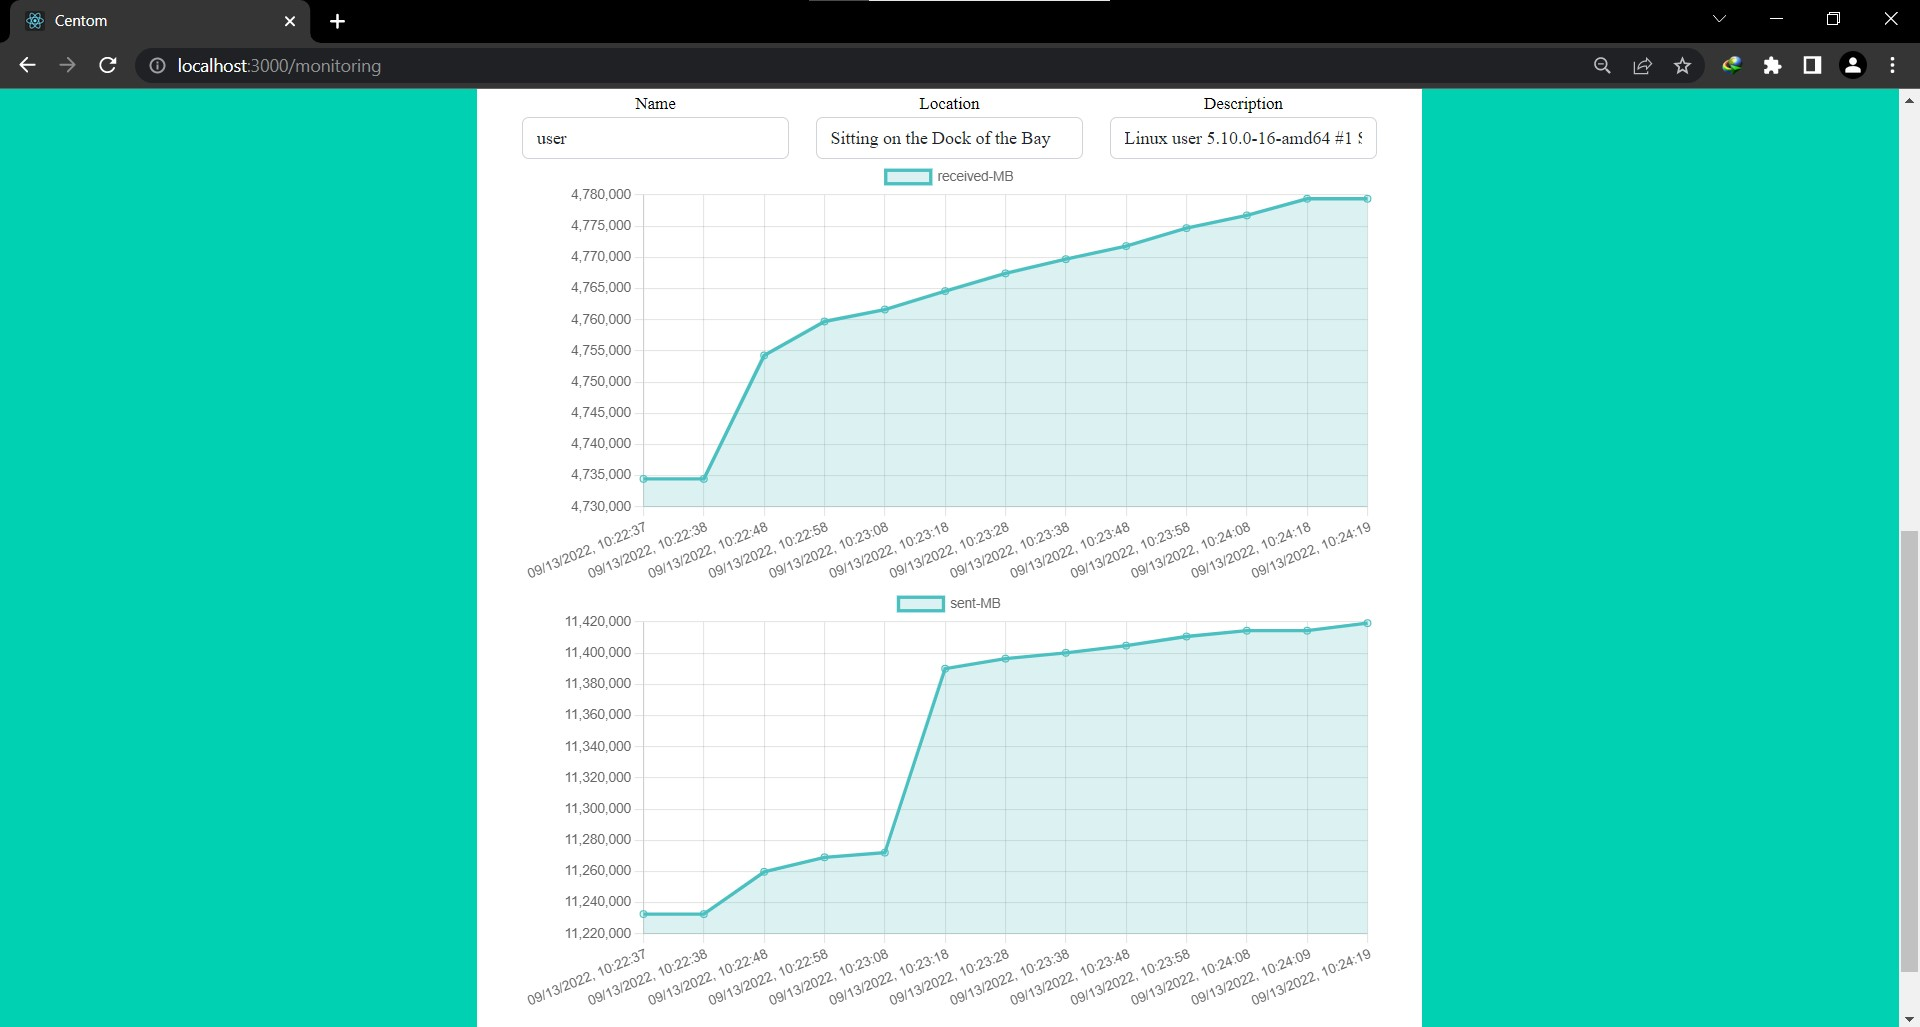
\includegraphics[scale=.38]{./monitoring-before}
    \caption{تصویر نمودارهای مربوط به پارامترها}\label{fig.53}
\end{figure}


\begin{figure}[!h]
    \centering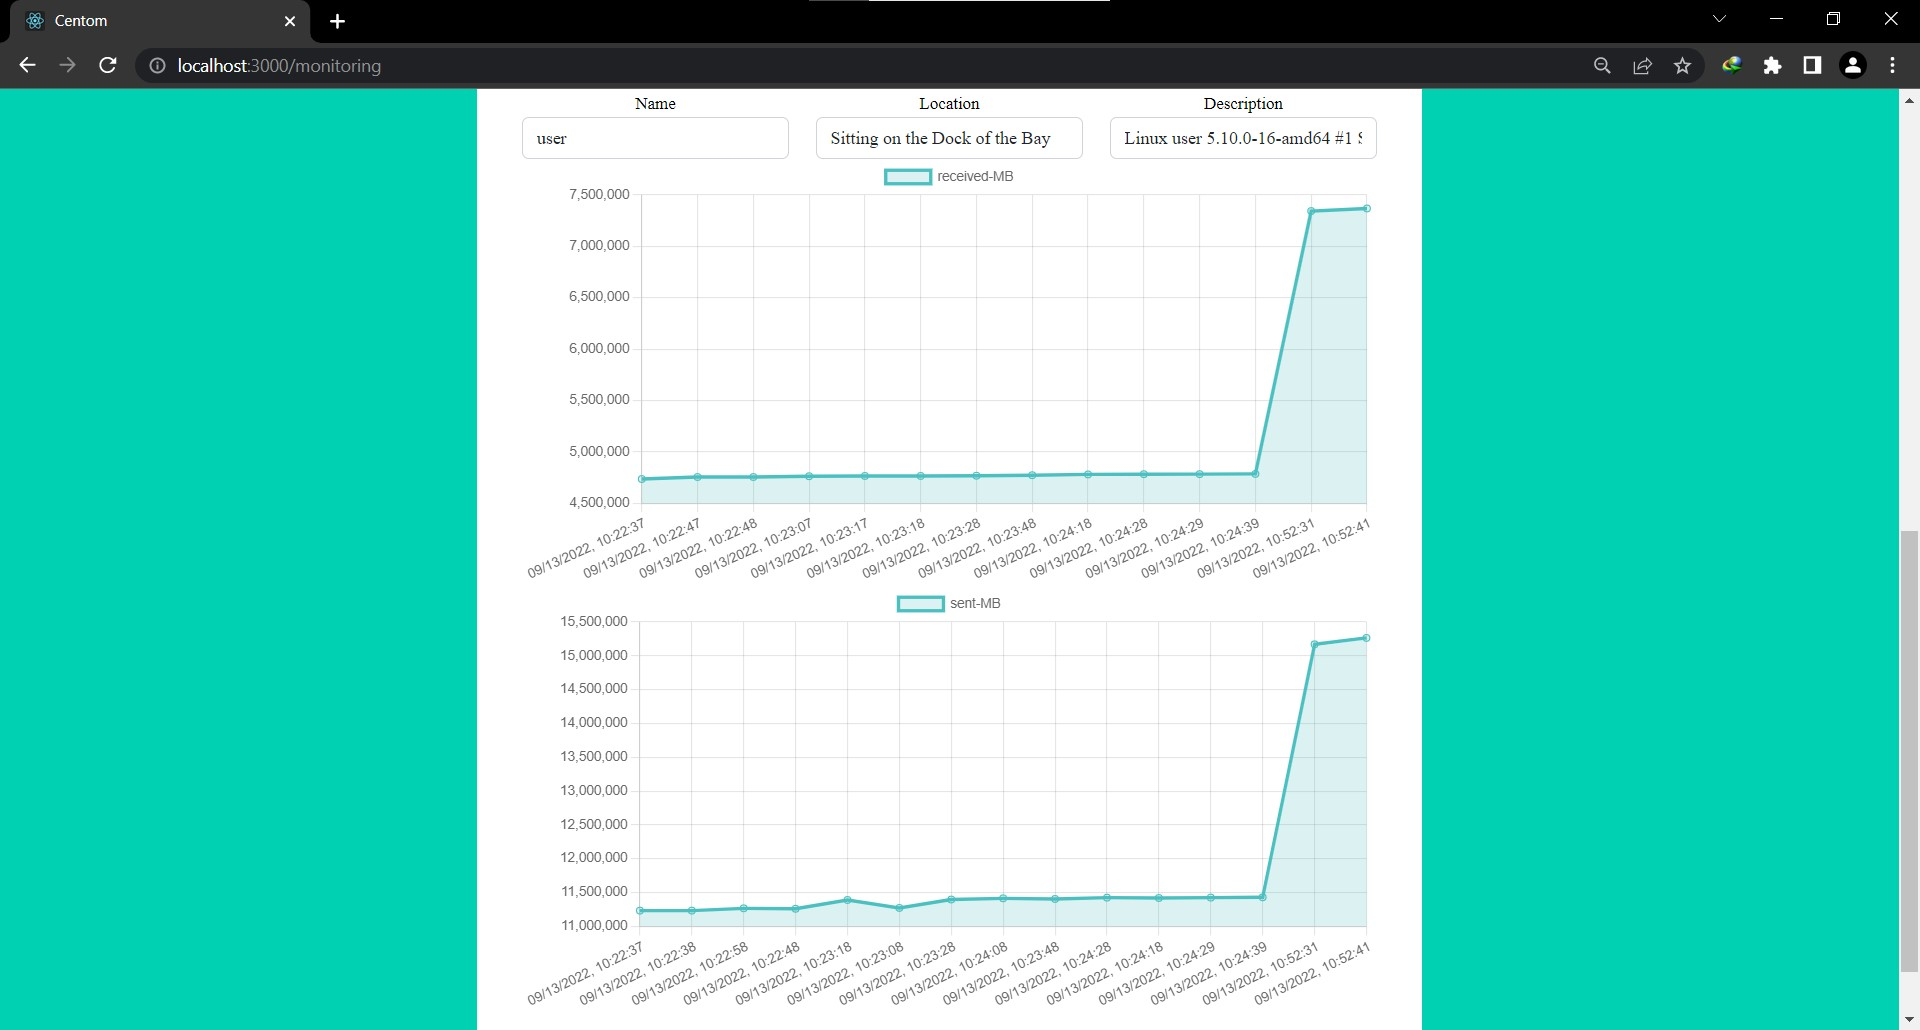
\includegraphics[scale=.38]{./monitoring-after}
    \caption{تصویر نمودارهای پارامترها جهت نمایش بازیابی صحیح اطلاعات}\label{fig.54}
\end{figure}

\cleardoublepage


\subsection{تست جمع‌آوری هشدارهای مربوط به عناصر تحت مدیریت}

برای این بخش از ابزار \lr{snmptrap} که تله‌ای مشخص می‌فرستد، استفاده شد. با این ابزار تله‌هایی طبق \cref{fig.55} به سامانه ارسال کرده و باید نتیجه در صفحه اعلانات بعد از فشردن دکمه مشاهده شود (به همان ترتیب و مقادیر)


همان‌طور که طبق \cref{fig.56} مشاهده می‌شود نتایج دقیقا با دستورات اجرایی مطابقت می‌نماید.


\begin{figure}[!h]
    \centering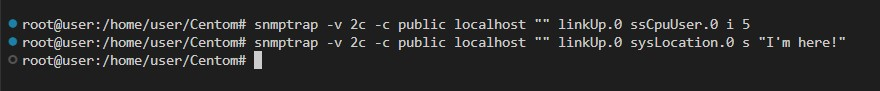
\includegraphics[scale=.70]{./trap-before}
    \caption{تصویر دستورات اجرا شده تله}\label{fig.55}
\end{figure}

\begin{figure}[!h]
    \centering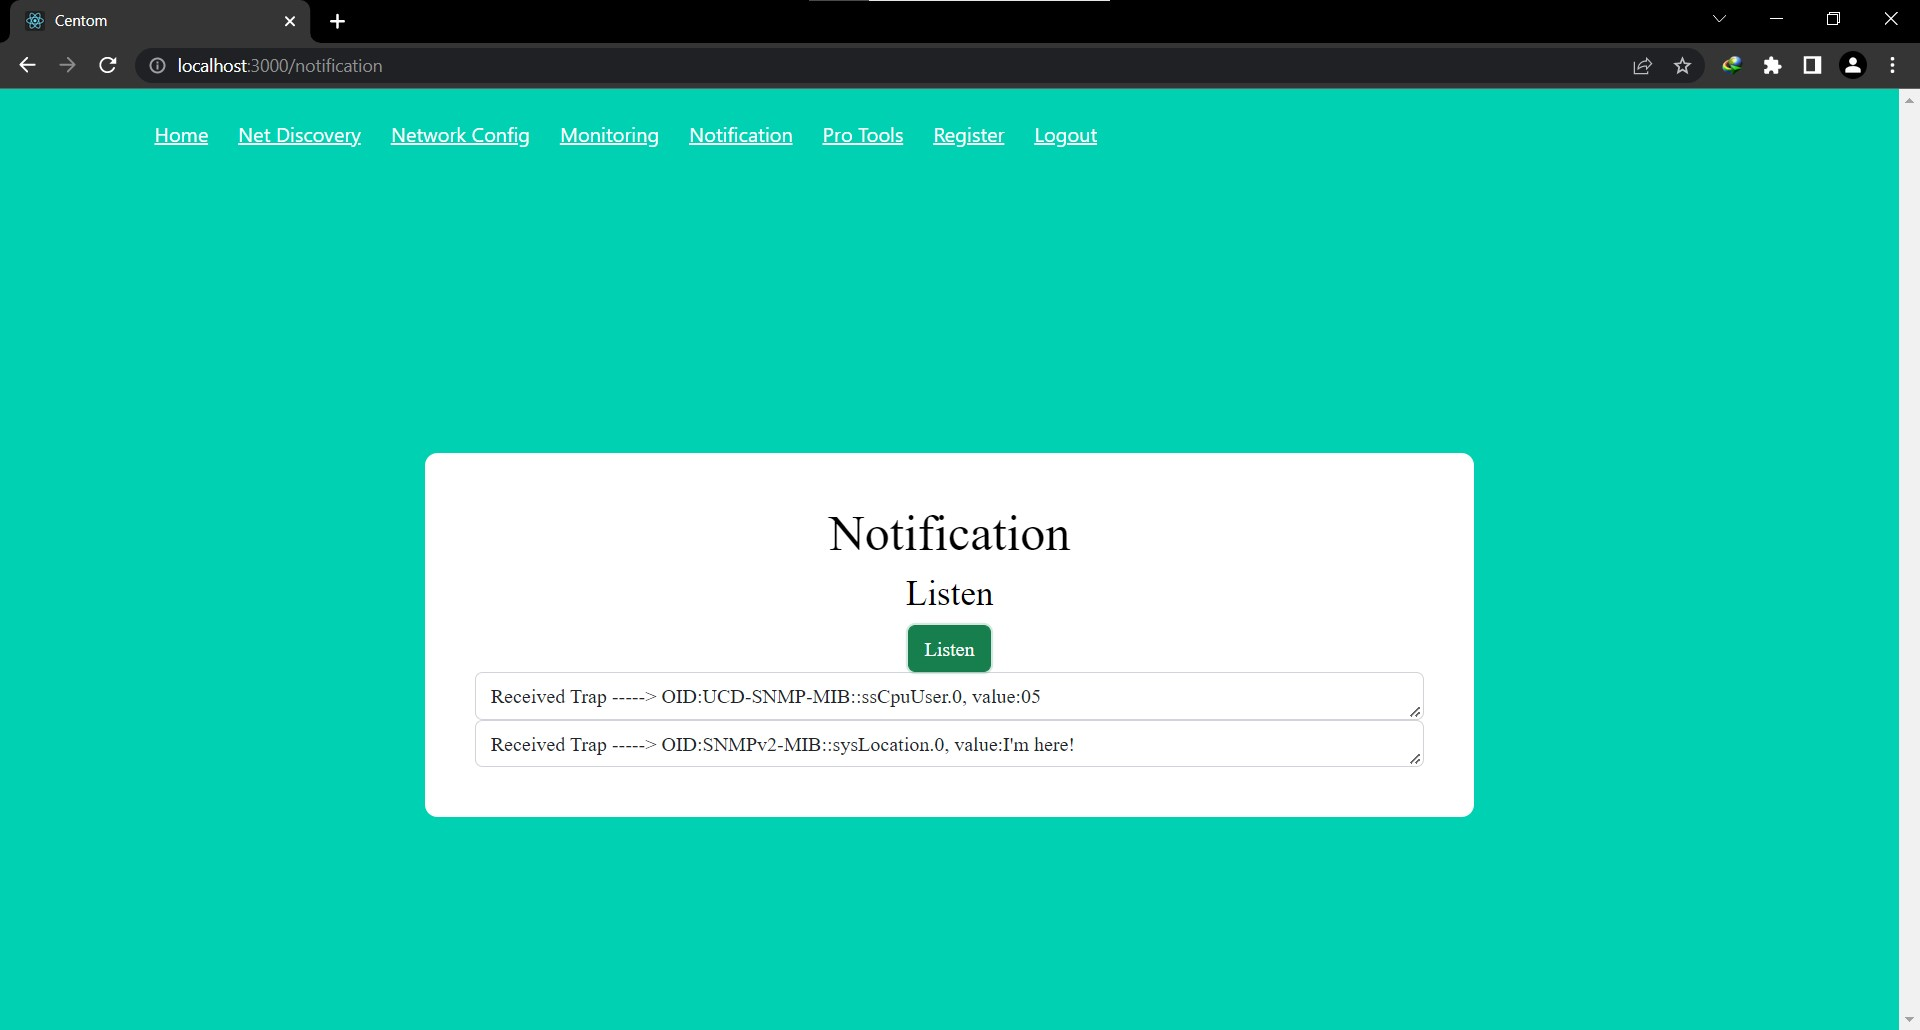
\includegraphics[scale=.38]{./notification}
    \caption{تصویر تله‌های دریافتی در سامانه}\label{fig.56}
\end{figure}

\cleardoublepage

\section{تست نیازمندی‌های غیرکارکردی}


\subsection{تست مدت زمان کشف شبکه}

دقیقا همان تستی که در بخش نیازمندی‌های کارکردی برای تست کشف شبکه انجام شد در مدت زمان  انجام شد. این مقدار کمتر از دو دقیقه (مقدار مطلوب) است.

\subsection{تست واسط کاربری مطلوب تحت وب}

پیاده‌سازی واسط کاربری این سامانه با چارچوب ری‌اکت و همچنین چارچوب فلسک در سمت سرور رابط کاربری مطلوبی را تحت وب برای افراد فراهم می‌آورد. همچنین برای استفاده از سامانه بیرون از شبکه سازمان، با چند تغییر تنظیمات در شبکه می‌توان به آن دسترسی پیدا کرد.

\subsection{تست امنیت سامانه }

در این قسمت برای ایجاد امنیت نسبی از چندین تکنیک به شرح استفاده شده است:

\begin{enumerate}
    \item استفاده از رمز عبور قوی برای دسترسی به هر دو پایگاه داده ردیس و \lr{SQLite} 
    \item استفاده از پروتکل \lr{SNMPv3} برای جمع‌آوری اطلاعات (پایش) که امنیت بهتری نسبت به ورژن دو فراهم می‌آورد
    \item استفاده از فایل تنظیمات خارج از کد پروژه که دسترسی به رمز عبورها سخت‌تر شود

\end{enumerate}